\documentclass{ucb}
\usepackage{cleveref}

\newcommand{\WMLES}{\textup{WMLES}}
\newcommand{\RANS}{\textup{RANS}}
\newcommand{\LES}{\textup{LES}}
\newcommand{\DDES}{\textup{DDES}}
\newcommand{\IDDES}{\textup{IDDES}}
\newcommand{\Ret}{\Re_\tau}

\begin{document}
\ucbcourse{\textbf{ASEN 6037} Turbulent Flows}
\ucbtitle{Literature Review: \textit{A Hybrid {{RANS}}-{{LES}} Approach with Delayed-{{DES}} and Wall-Modelled {{LES}} Capabilities}}
\ucbauthors{James Wright \\}
\ucblocation{Boulder, Colorado}
\ucbcover{}

\section{Introduction}
This literature review will cover the content and background of \citetitle{shurHybridRANSLESApproach2008}\cite{shurHybridRANSLESApproach2008}. 

\section{Overview of Prior Work}
This paper introduces a new hybrid RANS-LES turbulence model, later known as the improved delayed detached eddy simulations (IDDES). Before reviewing the paper, let's review the history of hybrid turbulence models in general.

IDDES can trace it's main roots back to the seminal detached eddy simulation (DES)~\cite{SpalartP.R.JouW-H.StreletsM.Allamaras1997} model, first proposed by \citeauthor{SpalartP.R.JouW-H.StreletsM.Allamaras1997}. The concept and motivation of hybrid models is fairly simple. LES is very expensive (particularly near the wall) for high Re flows, while RANS is significantly cheaper but not reliably accurate for many types of flow problems. Hybrid models combine the two to exploit their strengths and cover up their weakness. In general, RANS is responsible for flow regions that are very expensive for LES (namely near the wall) and LES is responsible for regions where RANS is not adequate. This is visually shown in \cref{fig:HRLMS}, where the shaded regions represent the parts of the turbulent spectrum that are modeled.

\begin{figure}[h]
    \centering
    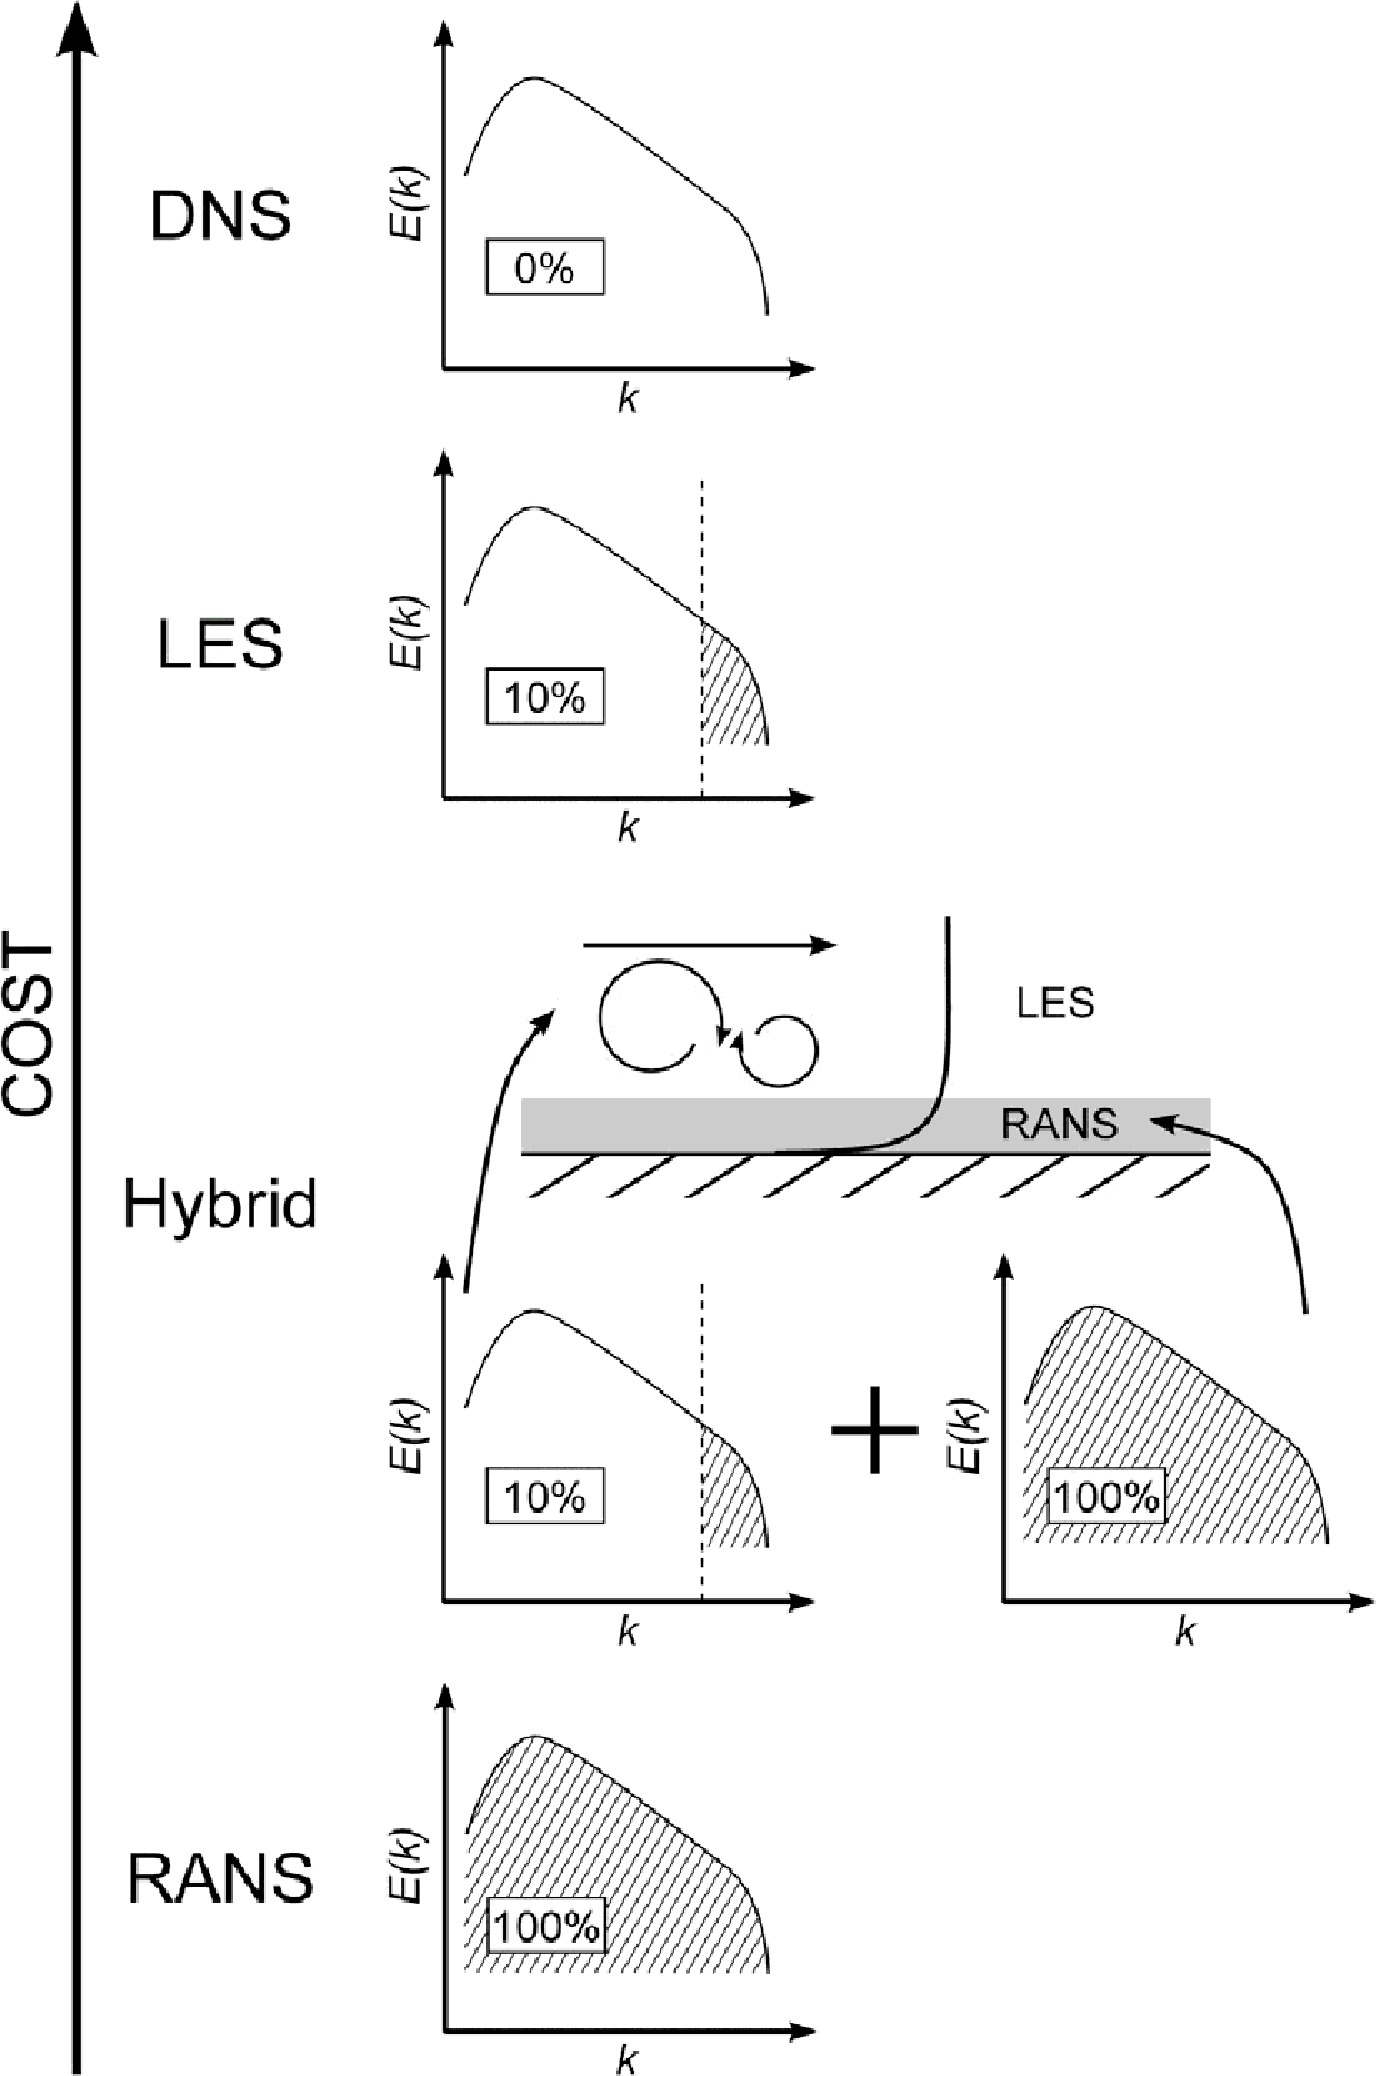
\includegraphics[]{img/TurbulenceModelsResolution_Tucker2015.jpg}
    \caption{Turbulence model hierarchy. Reproduced from~\cite{Tucker2015} under the Creative Commons Attribution License (\url{https://creativecommons.org/licenses/by/4.0/}).}
    \label{fig:HRLMS}
\end{figure}

% While there are some conceptual issues with the original DES formulation, %! reference to desire for WMLES instead of RANS near wall
The transition between the two models is one of the primary achilles's heel of DES-like methods. This is true both in determining where transition should occur and in transforming the modeled stress in the RANS region into resolved turbulence structures required by LES. The transition point was the primary reason for the first (of many) modifications to the original DES model. The DES model based the transition point on the grid size. This lead to issues (Modeled Stress Depletion and consequently Grid Induced Separation) when the model was used on different sized near-wall grids. This issue was addressed by \citeauthor{Menter2002} in \citedate{Menter2002} by introducing a shielding function to the DES formulation~\cite{Menter2002}. The original transition mechanism in DES was suppressed inside a boundary layer, as determined by the shielding function. This idea was originally only implemented with the SST-based DES model, but was generalized into the delayed detached eddy simulation (DDES) by \citeauthor{Spalart2006} in \citedate{Spalart2006}~\cite{Spalart2006}. 

The implementation of DES and DDES methods are based on an underlying RANS model. For the RANS ``mode'', the RANS model is essentially left alone. For the LES ``mode'', they adjust a turbulence length-scale parameter in the RANS model such that it only produces eddy-viscosity on the order of the SGS stresses. Thus, the DES and DDES models control the switch from RANS to LES via a turbulent length-scale parameter in the RANS model. DDES defines its length scale as 

\begin{equation}\label{eq:ellDDES}
    \ell_{\DDES} = \ell_{\RANS} 
    - f_d \max \left \{ 0, \left(\ell_\RANS - \ell_\LES \right) \right\}
\end{equation}

where \(f_d \) is a delaying function that controls where the transition occurs, and \(\ell_\LES \) and \(\ell_\RANS \) are the computed length scales need for ``pure'' LES and RANS mode respectively. \(f_d \) uses the sum of molecular viscosity \(\nu \) and eddy viscosity \(\nu_t \) as an input. This will be an important detail in the discussion of IDDES.

There have been attempts to use DES as a wall-modeled LES (WMLES), where RANS is used for modeling turbulence in a thin region within the boundary layer. However, at the transition between the RANS and LES regions, there exists what is known as the log-layer mismatch, referring to the log-law portion of the boundary layer. The issue is that while both RANS and LES both accurately predict the logarithmic relationship between \(u^+\) and \(y^+\), they predict them at different magnitudes. Thus, at the boundary between then, the velocity profile must transition from the log-law relationship predicted by RANS to the one predicted by LES.

\section{Work Summary}
This work introduces a new hybrid RANS-LES turbulence model dubbed the improved delayed detached eddy simulation (IDDES). The goal of the model is to allow for WMLES and standard DDES operation in the same model. Additionally, it aims to resolve the log-layer mismatch seen in other applications of DES-esque models for WMLES.
%TODO Add sentence regarding things to be reviewed. ie:
% To achieve this, a new subgrid length-scale was developed, in addition to the chagnes to the model euqations themselves.

\subsection{Subgrid Length-Scale}
The first major part introduced in the paper is a new definition for the subgrid length-scale, \(\Delta \). Traditionally, this is approximated by either the cube root of the element/cell volume or by the maximum of three element/cell spacings, \(h_{\max} \). Most SGS models use \(\Delta \) as a significant input to their calculation. However, the problem with either of these definitions is that the model coefficients for SGS model in near-wall flows is significantly different for free stream flows. Ideally, the SGS model coefficients should constant regardless of their location in the flow. To achieve this, \citeauthor{shurHybridRANSLESApproach2008} created a new definition of \(\Delta \) that used wall distance, \(d_w \), as an input. Far from the wall, \(\Delta \) should be equal to \( h_{\max} \). Close to the wall, \(\Delta \) should be made some function of the wall-parallel spacings. Ignoring the wall-normal spacing is done to avoid the sharp changes in the wall-normal spacing common with meshes close to the wall. To transition between these two extremes, it is assumed that \(\Delta \) is a linear function of \(d_w \). Lastly, it is also noted that \(\Delta \) should be constrained to be between the minimum and maximum wall spacings. The end result is

\begin{equation}\label{eq:delta}
    \Delta = \min \left \{ 
        \max \left \{ C_w d_w, C_w h_{\max}, h_{wn}\right \} 
        , h_{\max} \right \}
\end{equation}
where \(C_w\) is a constant, which was found to be 0.15, and \(h_{wn} \) is the wall-normal grid spacing. The latter argument of the min function gives the behavior far from the wall while the max function (within the min function) gives the behavior near the wall.
The two features of the above definition are that \(\Delta \) is reduced in the near-wall region and transitions to the ``free-stream'' value quickly. 

%TODO come back and add the actual results

\subsection{IDDES Model Equations}
IDDES is made up of two primary ``modes''; a DDES mode and a WMLES mode. These different modes are defined by the model with different turbulent length scales. The length scale for DDES is the same as presented in \cref{eq:ellDDES}.
The length-scale for the WMLES mode is give by:

\begin{equation}\label{eq:ellWMLES}
    \ell_\WMLES = f_B (1+f_e) \ell_\RANS + (1-f_B)\ell_\LES
\end{equation}

\(f_B \) is the primary determinant of where the RANS (\(f_B =1\)) to LES (\(f_B = 0\)) transition occurs and is a function of \(d_w / h_{\max} \).
The elevating function \(f_e \), unlike \(f_d \) or \(f_B \), can actually take values greater than one, and thus increase (ie. ``elevate'') the value of \(\ell_\RANS \). It is present to ensure that the RANS stresses are not disposed of prematurely when transitioning to LES mode. According to \citeauthor{shurHybridRANSLESApproach2008}, \(f_e \) ``is instrumental in combating log-layer mismatch'' \cite{shurHybridRANSLESApproach2008} \(f_e \) should equal to 0 (thereby leaving \(\ell_\RANS \) present in the calculation of \(\ell_\WMLES \) as the dominant term) when the grid is not sufficient to resolve the dominant wall-eddies of the flow \textit{and} when the pure RANS mode is desired. In the cases where \(f_e \) is not zero, it may be larger than 1, where it can compensate for \(f_B \) decreasing too close to the wall.

These two separate modes are combined in the following way. First, \(f_d \) is redefined slightly differently as

\begin{equation}
    \tilde{f}_d = \max \left\{ 1- f_{dt}, f_B \right\}
\end{equation}

where \(f_{dt} \) is a function of \(\nu_t \) (recall that the original \(f_d \) was a function of \(\nu + \nu_t \)). This adjusted \(\tilde{f}_d \) can then be placed into the expression for \(\ell_\WMLES \) found in \cref{eq:ellWMLES}. This gives us the final expression for the IDDES length scale:

\begin{equation}\label{eq:ellIDDES}
    \ell_\IDDES = \tilde{f}_d (1 + f_e) \ell_\RANS + (1 - f_B) \ell_\LES
\end{equation}


\subsection{Simulations}

To prove the efficacy of the new \(\Delta \) definition, simulations were done using \(\Delta \)on a plane channel flow for wall-resolved LES (WRLES) and WMLES. The WRLES simulation was performed at \(\Ret = 400 \) and showed much better results than using \(\Delta = \textup{Vol}^{1/3} \). 
The WMLES was done at  \(\Ret = 1100 \) and \(\Ret = 18000 \). The results for \(\Ret = 18000 \) were quite good, but at \(\Ret = 1100\) the new definition for \(\Delta \) was not able to accurately predict the log-law region of the boundary layer. Overall though, this is a significant improvement as there was not log-layer mismatch using the new \(\Delta \).

To test the IDDES model two different batches of simulations were used. Channel flow and a hydrofoil in shallow stall were used to test the WMLES capabilities of the IDDES model, while backwards facing step was shown to test the DES/DDES mode of the model. Understandably, most of the emphasis and analysis of the paper was put into to the WMLES results. The results shown used the \(k \) - \(\omega \) shear stress transport (SST) model~\cite{Menter1994} as the underlying turbulence model, but reportedly the results were very similar for using the Spalart-Allmaras model~\cite{spalartOneequationTurbulenceModel1992}. 

For the channel WMLES simulations, analysis was done of not only the overall model performance, but also looking at the behavior of the various functions used in the model (\(f_B \), \(f_e \), \(f_{dt}\), etc.). Overall, the the channel flow showed that the IDDES model used in WMLES model was able to avoid log-layer mismatch, retain resolved turbulent content at small wall distances, and transition rapidly from RANS to LES at the correct location in comparison to DDES. It was also shown to be relatively robust to changes in grid size; effectively moving the RANS to LES transition to a location such that no loss in  wall stress was observed and not log-layer mismatch was observed. For the shallow separating hydrofoil, IDDES shows a quick transition to resolved turbulence in the separation, a known deficiency with DDES, and also predicts velocity magnitude and fluctuation profiles well in the attached and separated regions of the flow.

The backwards facing step simulation showed that the IDDES model works exactly as expected; RANS is used in on the top of the step where no turbulent content exists, LES is used in the separation region, and WMLES is used in the reattachment regime downstream of the step. The results of the actual flow itself were also quite good, where the IDDES outperformed both DDES and RANS when compared with experimental results.

\subsection{Comments on Results}
The IDDES model presented in this work represents as significant step forward in the accuracy and capabilities of hybrid RANS-LES turbulence models. While previous models, namely DES and DDES, were quite good with massive/geometry-induced flow separation, their performance in shallow separation and attached boundary layers was less than ideal. They were often slow to transition to a resolved state or they would fail to predict flow separation all together. IDDES, with it's integration of a WMLES mode, allows for much better prediction of the shallow separation regions while retaining the behavior and accuracy of DES/DDES in regions of massive separation or no resolved turbulent content.

%* Problems with the model: See the Riccardo ZDES paper

\section{Potential Issues}
One of the immediate potential issues I see is the grid dependence of \(f_B \) and \(f_e \) in the WMLES mode of IDDES. Their dependence on grid size leads back to the exact issues with the original DES and modeled stress depletion. At the end of the day, these functions are meant to determine where the the log-layer ends and to start using WMLES at that location. The wall distance location of the log-layer is not inherently a grid dependent quantity and thus, in my opinion, functions attempting to model that distance should not be a function of any grid parameters. That being said, I'm sure this is an issue the authors are quite aware of and this model is a result of a multitude of compromises.

Another major caveat to IDDES is that, for adverse pressure gradient induced stall, it is still reliant on RANS for the prediction of flow separation. While this is far from terrible, it's also not ideal either, as the RANS is not a great predictor of these regions. 
In particular, RANS is poor in rapid changes in pressure gradients, such as at the leading edge of an airfoil or a bump. 
When acting in WMLES mode, these issues are less significant as only the inner layer of the boundary layer is being handled by RANS. However, there may still be issues present with it's implementation. 

% Additionally, the usage of \(\nu_t \) in the determination of where the transition should occur may be problematic. In fact this was discovered later on.
% cite entropy papers "Towards an entropy-based detached-eddy simulation

% Conversely, I don't see any significant issues with the grid dependence of \(\Delta \) as it is inherently grid dependent due to the relationship between the implicit LES filter width and the grid size. 

\section{New Questions}
The obvious question coming from both my comments on potential issues and the proceeding literature is whether there is a better way to determine the transition locations for RANS-LES hybrid models, be them in a traditional DES or WMLES sense.

\ucbbib{}
    
\end{document}
